%!TEX root = ../thesis.tex

\section{実験概要}
本章では, 前章の実験で使用した教師データに問題があるかを調査するために, 2種類の実験を行う. 1つ目は教師データを入れ替えた実験, 2つ目はカメラを9個にした実験である. 前者の実験で, カメラ画像と目標角速度のどちらに問題があるかを明らかにする. 後者の実験では, 3つのカメラから得られる画像の切り抜きに問題があるかを確かめる. 

\section{実験方法}
まず初めに, 教師データを入れ替えた実験に関して説明する. \figref{Fig:change}のように, 5章で最も成功率の高かった実験(以後, 実験1と呼ぶ)で使用した教師データと, 前章の実験(以後, 実験2と呼ぶ)で使用した教師データを入れ替えて学習を行う.
\par 次に, カメラを9個にした実験について説明する. カメラの取り付け位置は, 前章の3つのカメラそれぞれを基準として, ヨー方向に±5[deg]回転させたカメラを追加する. このロボットを使用して, 走行させながらデータ収集を行う. 目標角速度に関しては, 前章のオフセットを用いる. 
\par 原因の調査を行うために, シミュレータを用いた実験を行う. 実験環境, 実験装置は前章と同様のシミュレータ環境を用いる.また, 学習器の訓練条件, 学習したモデルを用いたテストなどの条件は前章と同様とする. 実験条件は以下の通りである. 

\begin{description}
  \item[実験3] 実験1の目標角速度と実験2のカメラ画像の組み合わせ
  \item[実験4] 実験1のカメラ画像と実験2の目標角速度の組み合わせ
  \item[実験5] 実験1のカメラ画像と実験1の目標角速度の0[m], 0[deg]を\par \hspace*{6mm}実験2の目標角速度と入れ替え
  \item[実験6] 9個のカメラ画像と実験2のオフセットのパターン
\end{description}

\begin{figure}[h]
  \centering
  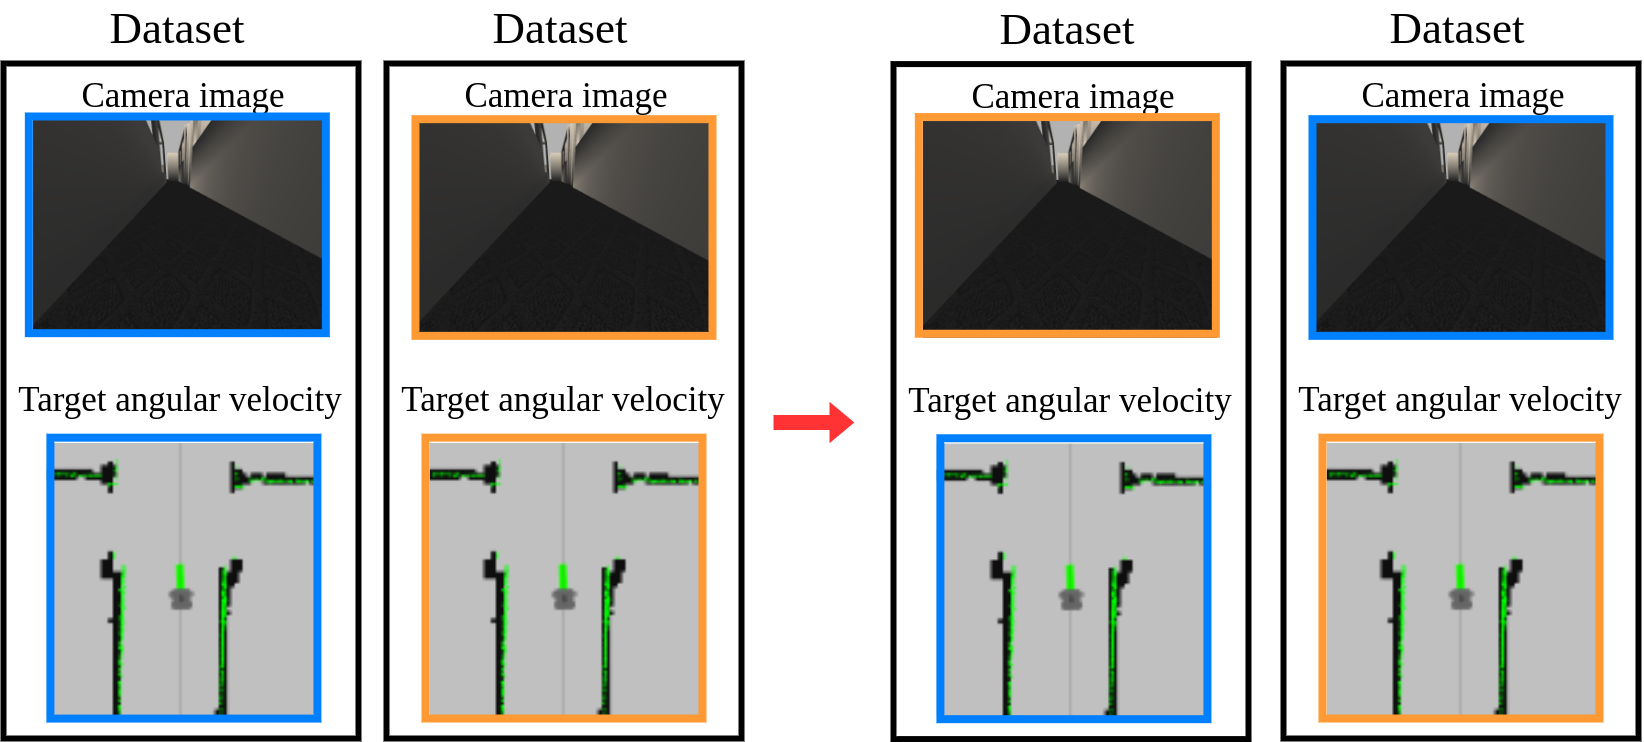
\includegraphics[keepaspectratio, scale=0.22]{images/change.png}
  \caption{Exchange of supervisory data}
  \label{Fig:change}
\end{figure}

\begin{figure}[h]
  \centering
  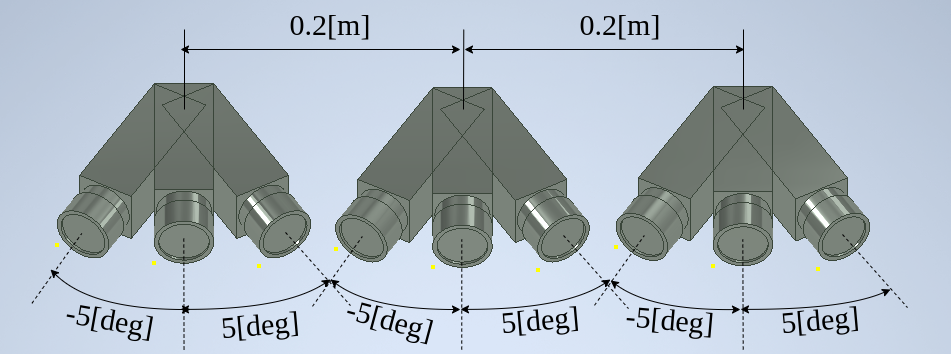
\includegraphics[keepaspectratio, scale=0.35]{images/9cam_draw.png}
  \caption{9cameras}
  \label{Fig:9cam}
\end{figure}

\newpage
\subsection{実験結果と考察}
実験結果を\tabref{tb:inves}に示す. 分母の30は実験回数を示しており, 分子の数は成功回数を示している. 結果的に, 実験3, 実験4, 実験6の成功回数はいずれも30回中0回, 実験5の成功回数は9/10となった. それぞれの実験の走行軌跡を\figref{Fig:fail3}, \figref{Fig:fail4}, \figref{Fig:fail5}, \figref{Fig:fail6}に示す. 失敗例は, 概ね実験2と同様に, 直進時に目標経路から外れて, 壁に衝突して失敗している. \figref{Fig:loss3}, \figref{Fig:loss4}, \figref{Fig:loss5},  \figref{Fig:loss6}に, 実験3, 実験4, 実験5, 実験6それぞれの条件で学習した際のlossのグラフを示す. 図から実験5のみ緩やかにlossが減少していることがわかる. それ以外は, 初期でlossが減少に急激して, その後は値がほぼ変化していないことが確認できる. 
\par 実験3の結果から, 実験2のカメラ画像1枚から3つの画像を切り抜く画像が, 実験1の画像と同じであれば, 実験3は経路追従できるはずである. 同様に, 実験4の結果から, 実験2のmove\_baseの出力を参考にオフセットを加えた目標角速度が, 実験1の目標角速度に近ければ経路追従できるはずである. 実験5からは, 実験2で収集した目標角速度には特に問題はなく, 経路追従を継続するには, 目標経路から±0.2[m]の位置, ヨー方向に±5[deg]の目標角速度が重要であると考えられる. 
\par これらのことから, カメラ画像から左右に切り抜く方法では, ロボットをヨー方向に±5[deg]回転させた際の画像を再現できていないと考えられる. また, 目標角速度に関しても, 実験1ではそれぞれの位置と向きでルールベース制御器の出力を取得していた. しかし, 実験2ではロボットを走行させながら収集した角速度に, オフセットを加えることで, 各位置と向きを考慮した目標角速度を生成している. この方法では, 経路追従を継続するのに必要な目標角速度を再現できていないと考えられる. 目標経路及び±0.2の位置, 0[deg]及び±5[deg]の向きに, ロボットを配置した際に得られるカメラ画像と目標角速度を, どのように再現するかは今後の課題としたい. 

\newpage
\begin{table}[h]
  \centering
  \caption{Number of successes in the experiments of simulator}
  \begin{tabular}{|c|c|} \hline
      Experiments & Number of successes \\ \hline
      Exp. 3 & 0/30 \\ \hline
      Exp. 4 & 0/30 \\ \hline
      Exp. 5 & 9/10 \\ \hline
      Exp. 6 & 0/30 \\ \hline
    \end{tabular}
  \label{tb:inves}
\end{table}

\begin{figure}[h]
  \begin{minipage}[b]{0.45\linewidth}
    \centering
    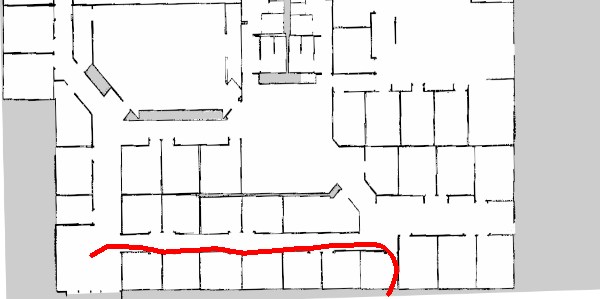
\includegraphics[keepaspectratio, scale=0.33]{images/exp3/traject30.png}
    \subcaption{}
  \end{minipage}
  \begin{minipage}[b]{0.45\linewidth}
    \centering
    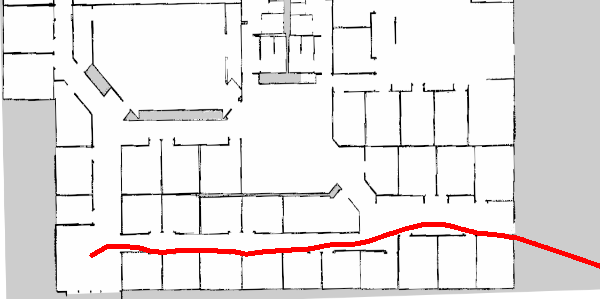
\includegraphics[keepaspectratio, scale=0.33]{images/exp3/traject25.png}
    \subcaption{}
  \end{minipage}
\caption{Example of failed path-tracking for experiment3}
\label{Fig:fail3}
\end{figure}

\begin{figure}[h]
  \begin{minipage}[b]{0.45\linewidth}
    \centering
    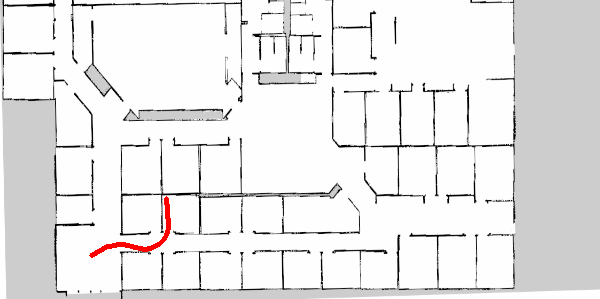
\includegraphics[keepaspectratio, scale=0.33]{images/00_02_rename/traject9.png}
    \subcaption{}
  \end{minipage}
  \begin{minipage}[b]{0.45\linewidth}
    \centering
    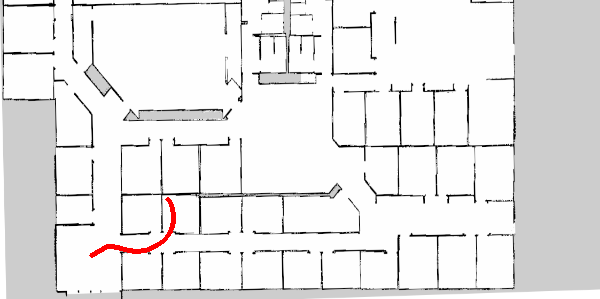
\includegraphics[keepaspectratio, scale=0.33]{images/00_02_rename/traject28.png}
    \subcaption{}
  \end{minipage}
\caption{Example of failed path-tracking for experiment4}
\label{Fig:fail4}
\end{figure}

\begin{figure}[h]
  \begin{minipage}[b]{0.45\linewidth}
    \centering
    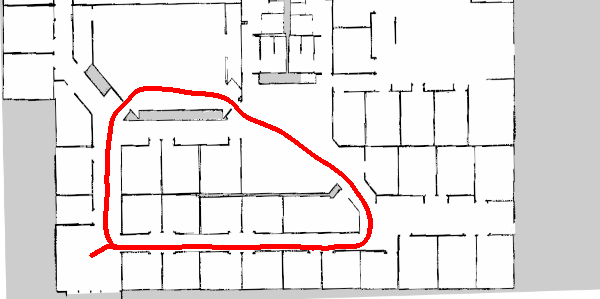
\includegraphics[keepaspectratio, scale=0.33]{images/mazemaze/traject1.png}
    \subcaption{}
  \end{minipage}
  \begin{minipage}[b]{0.45\linewidth}
    \centering
    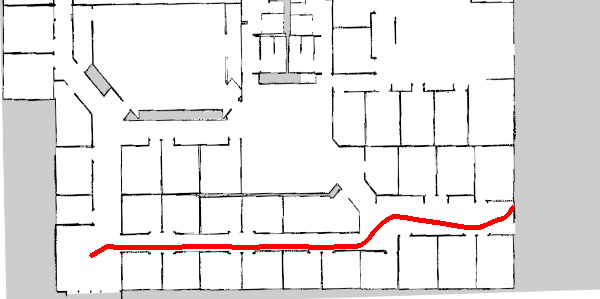
\includegraphics[keepaspectratio, scale=0.33]{images/mazemaze/traject8.png}
    \subcaption{}
  \end{minipage}
\caption{Example of successful and failed path-tracking for experiment5}
\label{Fig:fail5}
\end{figure}

\begin{figure}[h]
  \begin{minipage}[b]{0.45\linewidth}
    \centering
    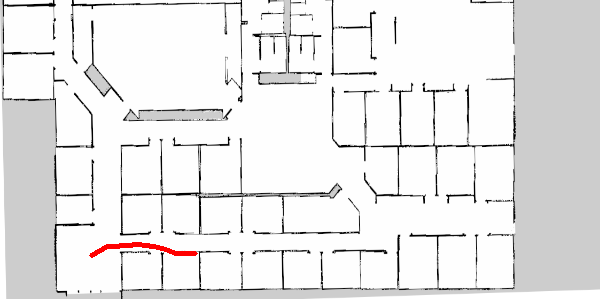
\includegraphics[keepaspectratio, scale=0.33]{images/9cam/traject19.png}
    \subcaption{}
  \end{minipage}
  \begin{minipage}[b]{0.45\linewidth}
    \centering
    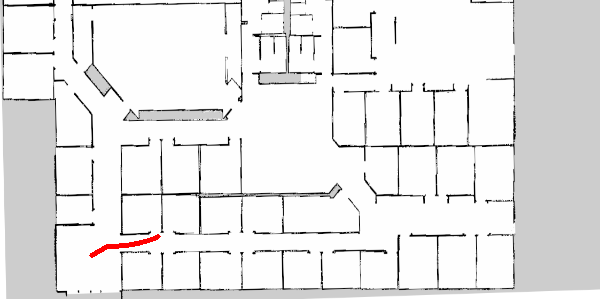
\includegraphics[keepaspectratio, scale=0.33]{images/9cam/traject26.png}
    \subcaption{}
  \end{minipage}
\caption{Example of failed path-tracking for experiment6}
\label{Fig:fail6}
\end{figure}

\begin{figure}[h]
  \centering
  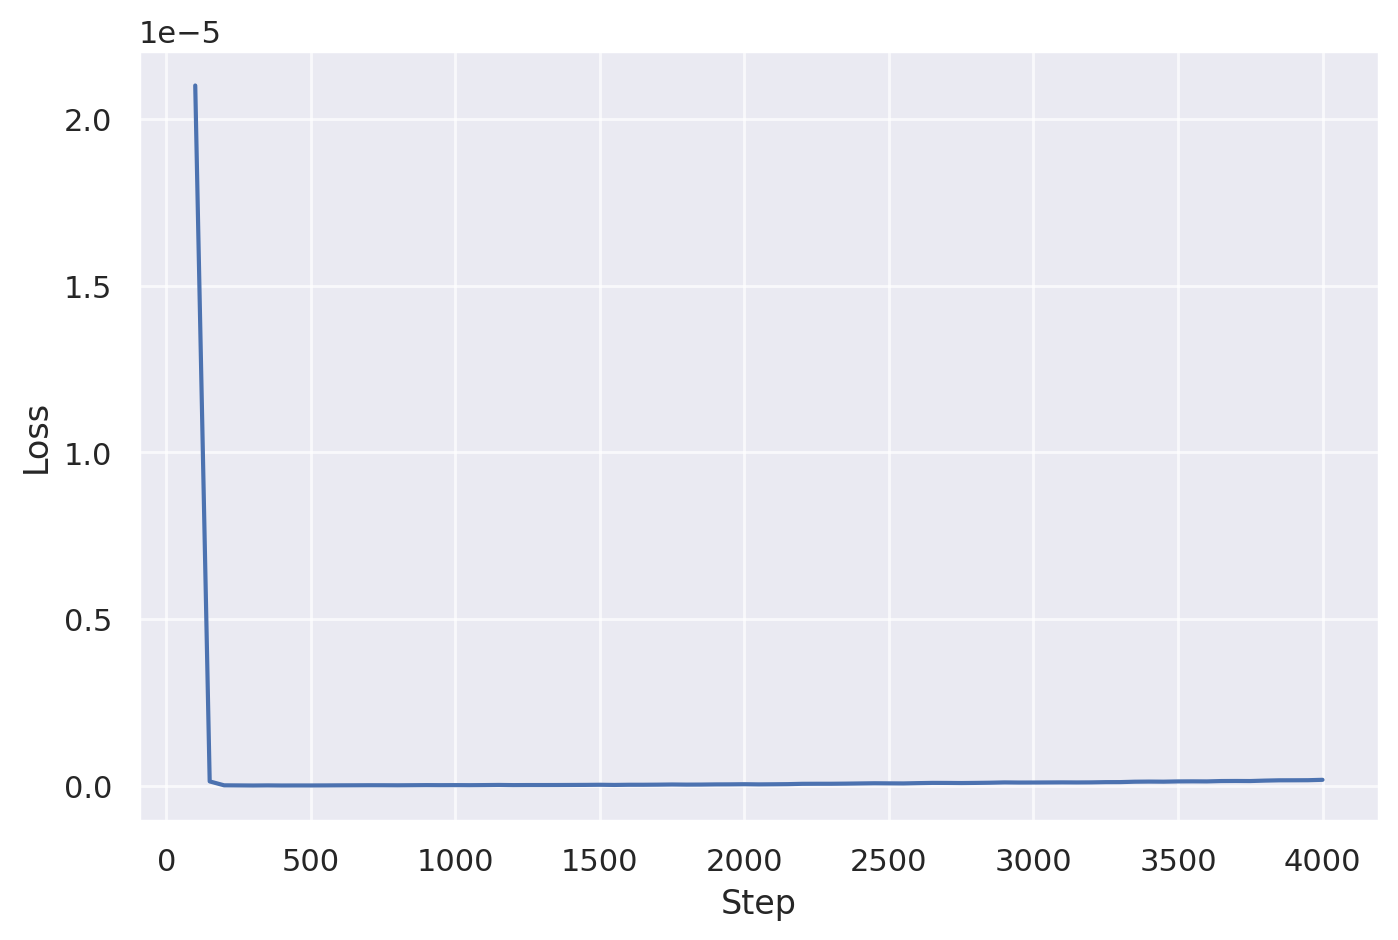
\includegraphics[keepaspectratio, scale=0.33]{images/exp3_25.png}
  \caption{Loss value in the experiment3}
  \label{Fig:loss3}
\end{figure}

\begin{figure}[h]
  \centering
  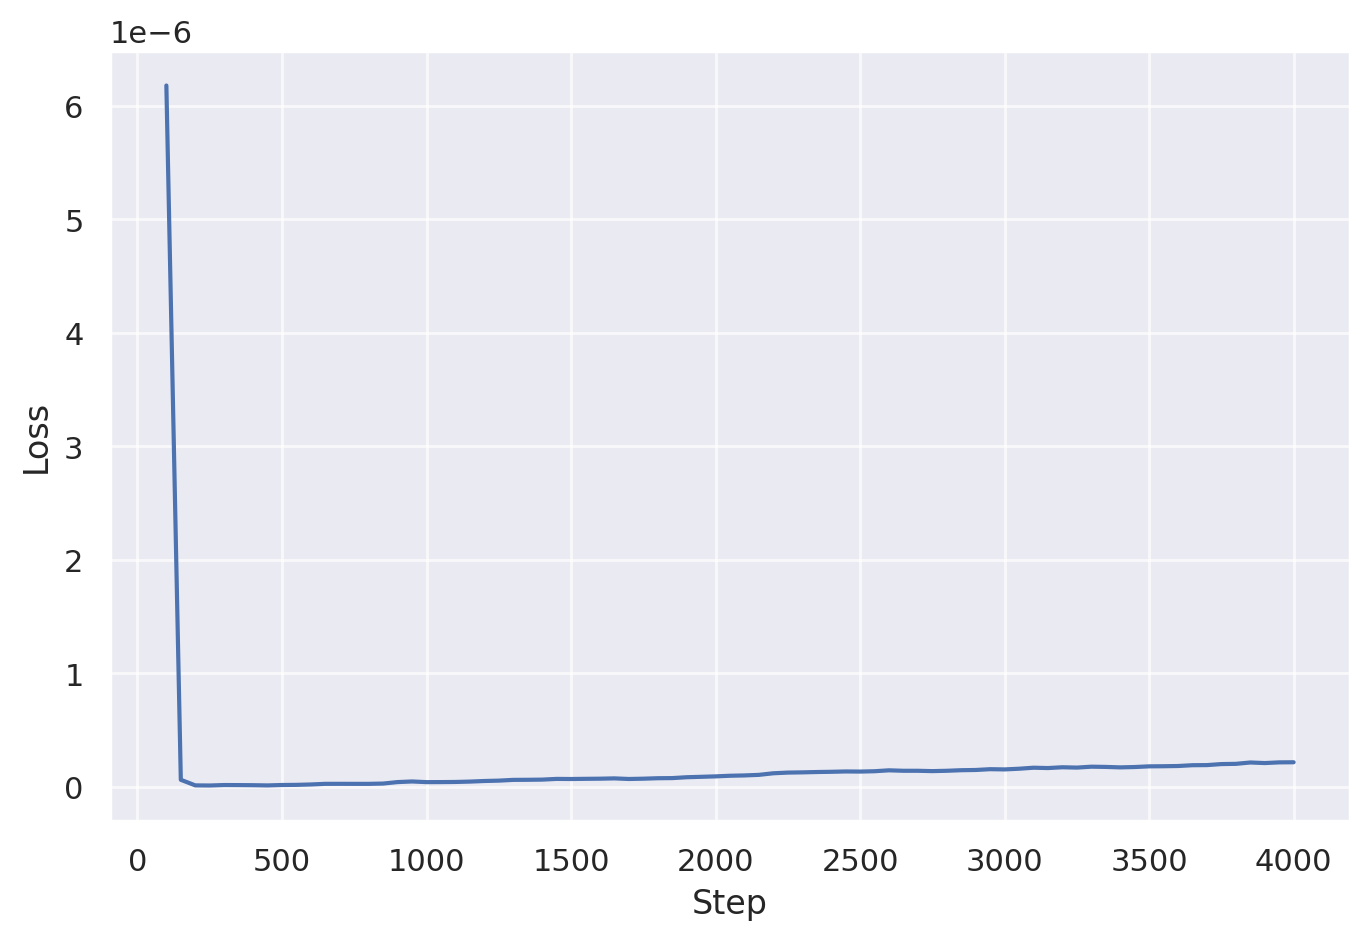
\includegraphics[keepaspectratio, scale=0.33]{images/00_02_rename_9.png}
  \caption{Loss value in the experiment4}
  \label{Fig:loss4}
\end{figure}

\begin{figure}[h]
  \begin{minipage}[b]{0.45\linewidth}
    \centering
    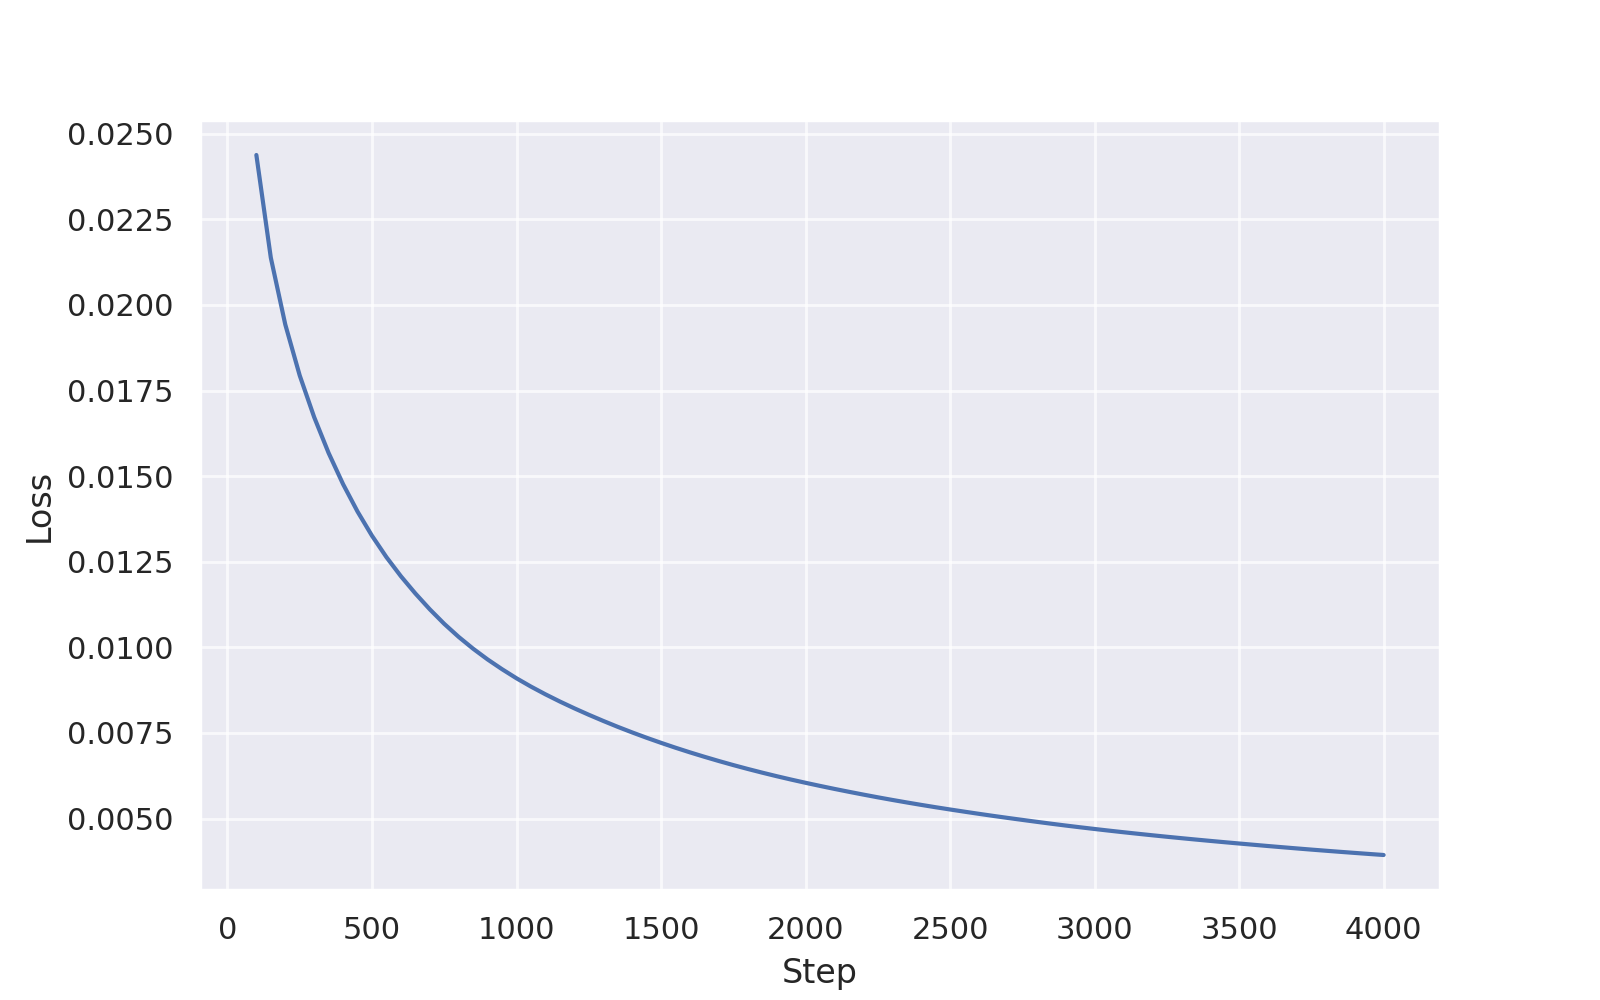
\includegraphics[keepaspectratio, scale=0.33]{images/mazemaze_1.png}
    \subcaption{}
  \end{minipage}
  \begin{minipage}[b]{0.45\linewidth}
    \centering
    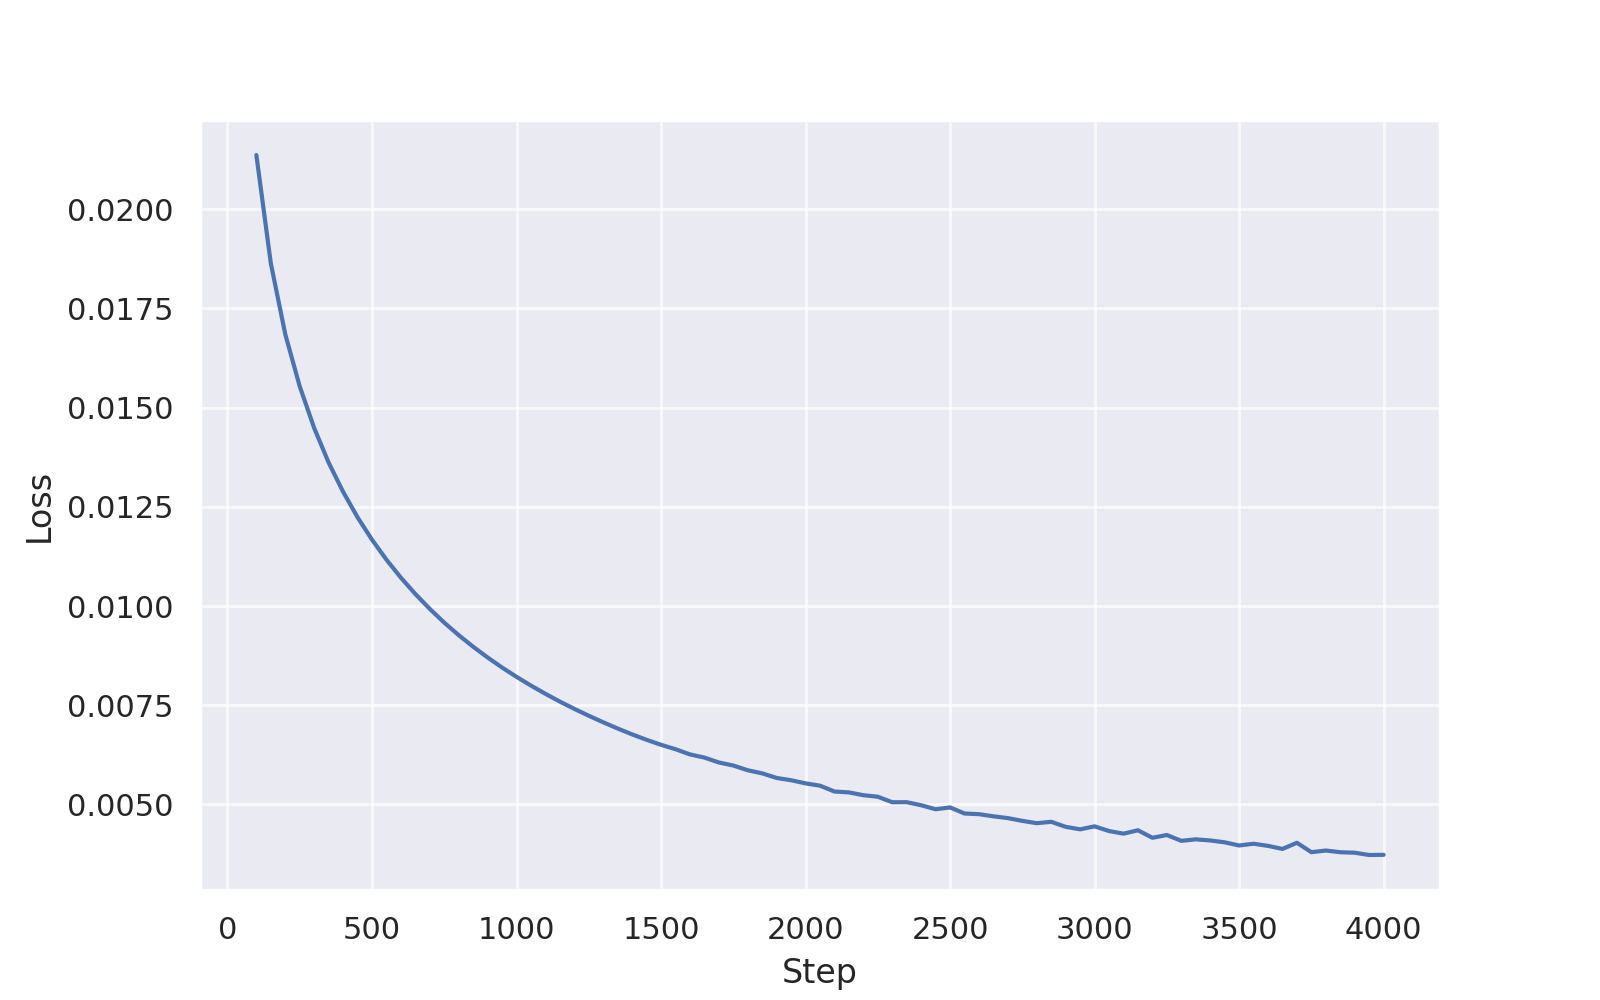
\includegraphics[keepaspectratio, scale=0.33]{images/mazemaze_8.png}
    \subcaption{}
  \end{minipage}
\caption{Loss value in the experiment5}
\label{Fig:loss5}
\end{figure}

\begin{figure}[h]
  \centering
  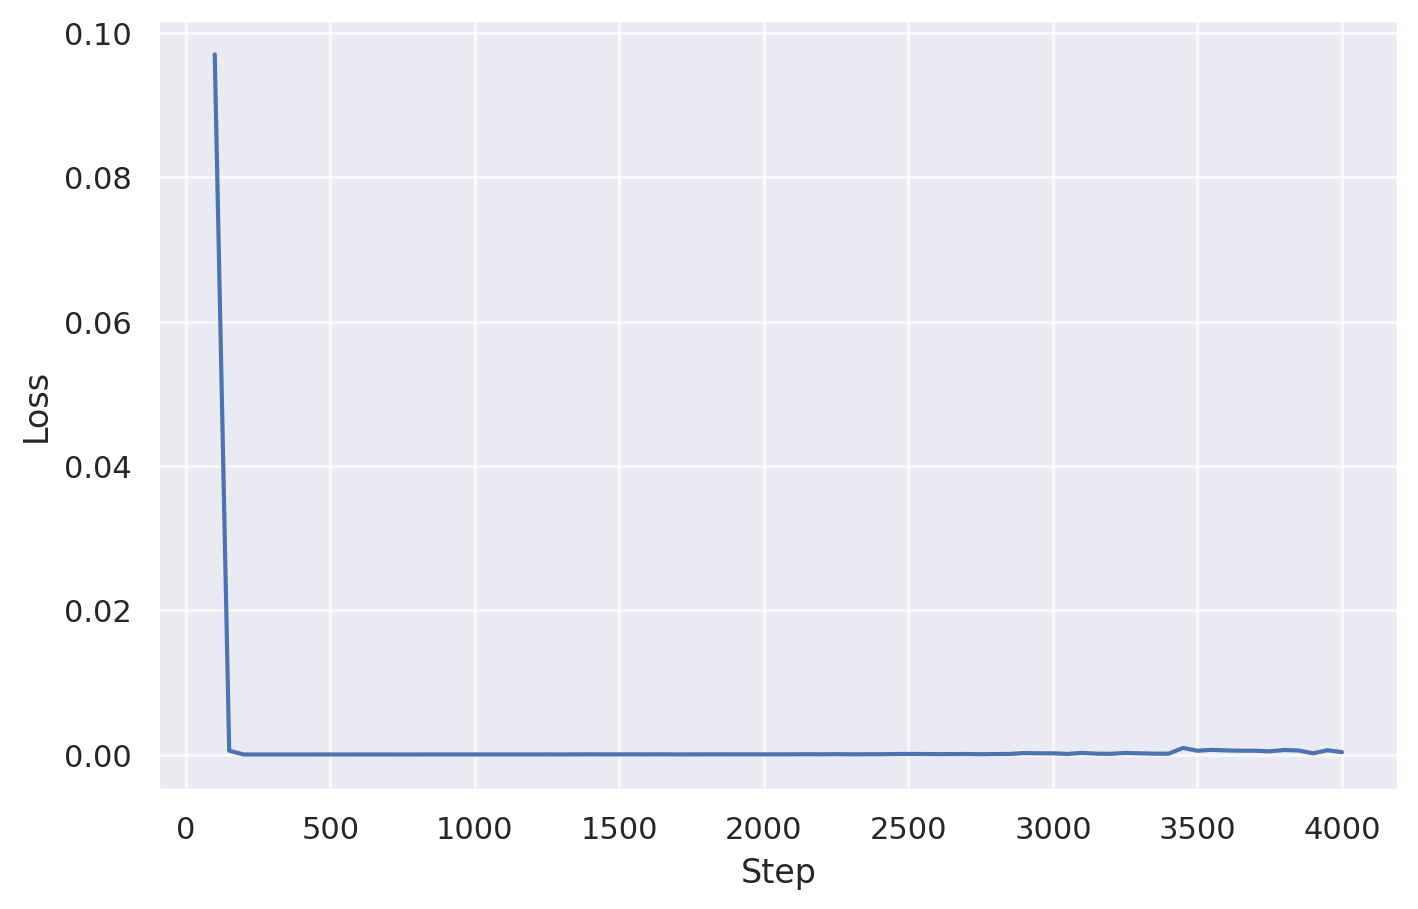
\includegraphics[keepaspectratio, scale=0.33]{images/9cam_19.png}
  \caption{Loss value in the experiment6}
  \label{Fig:loss6}
\end{figure}

\clearpage
\section{まとめ}
本章では, 前章の実験で使用した教師データに問題があるか調査を行った. シミュレータを用いた実験により, 以下のことを確認した.

\begin{itemize}
  \item 3つのカメラから得られる画像を切り抜く手法では, ロボットをヨー方向に±5[deg]回転させた際の画像を再現できていなく, 画像に問題があることを確認
  \item ロボットを走行させた際に得られる目標角速度に, オフセットを加えた値に問題があることを確認
\end{itemize}

% 前章で最も成功率の高かった際の教師データを実験1, 本章の教師データを実験2として比較を行う. これにより, 目標角速度とカメラ画像に問題があるかを調査する. \figref{Fig:ratio}に目標角速度の割合を比較したグラフを示す. 

% \begin{figure}[h]
%   \centering
%   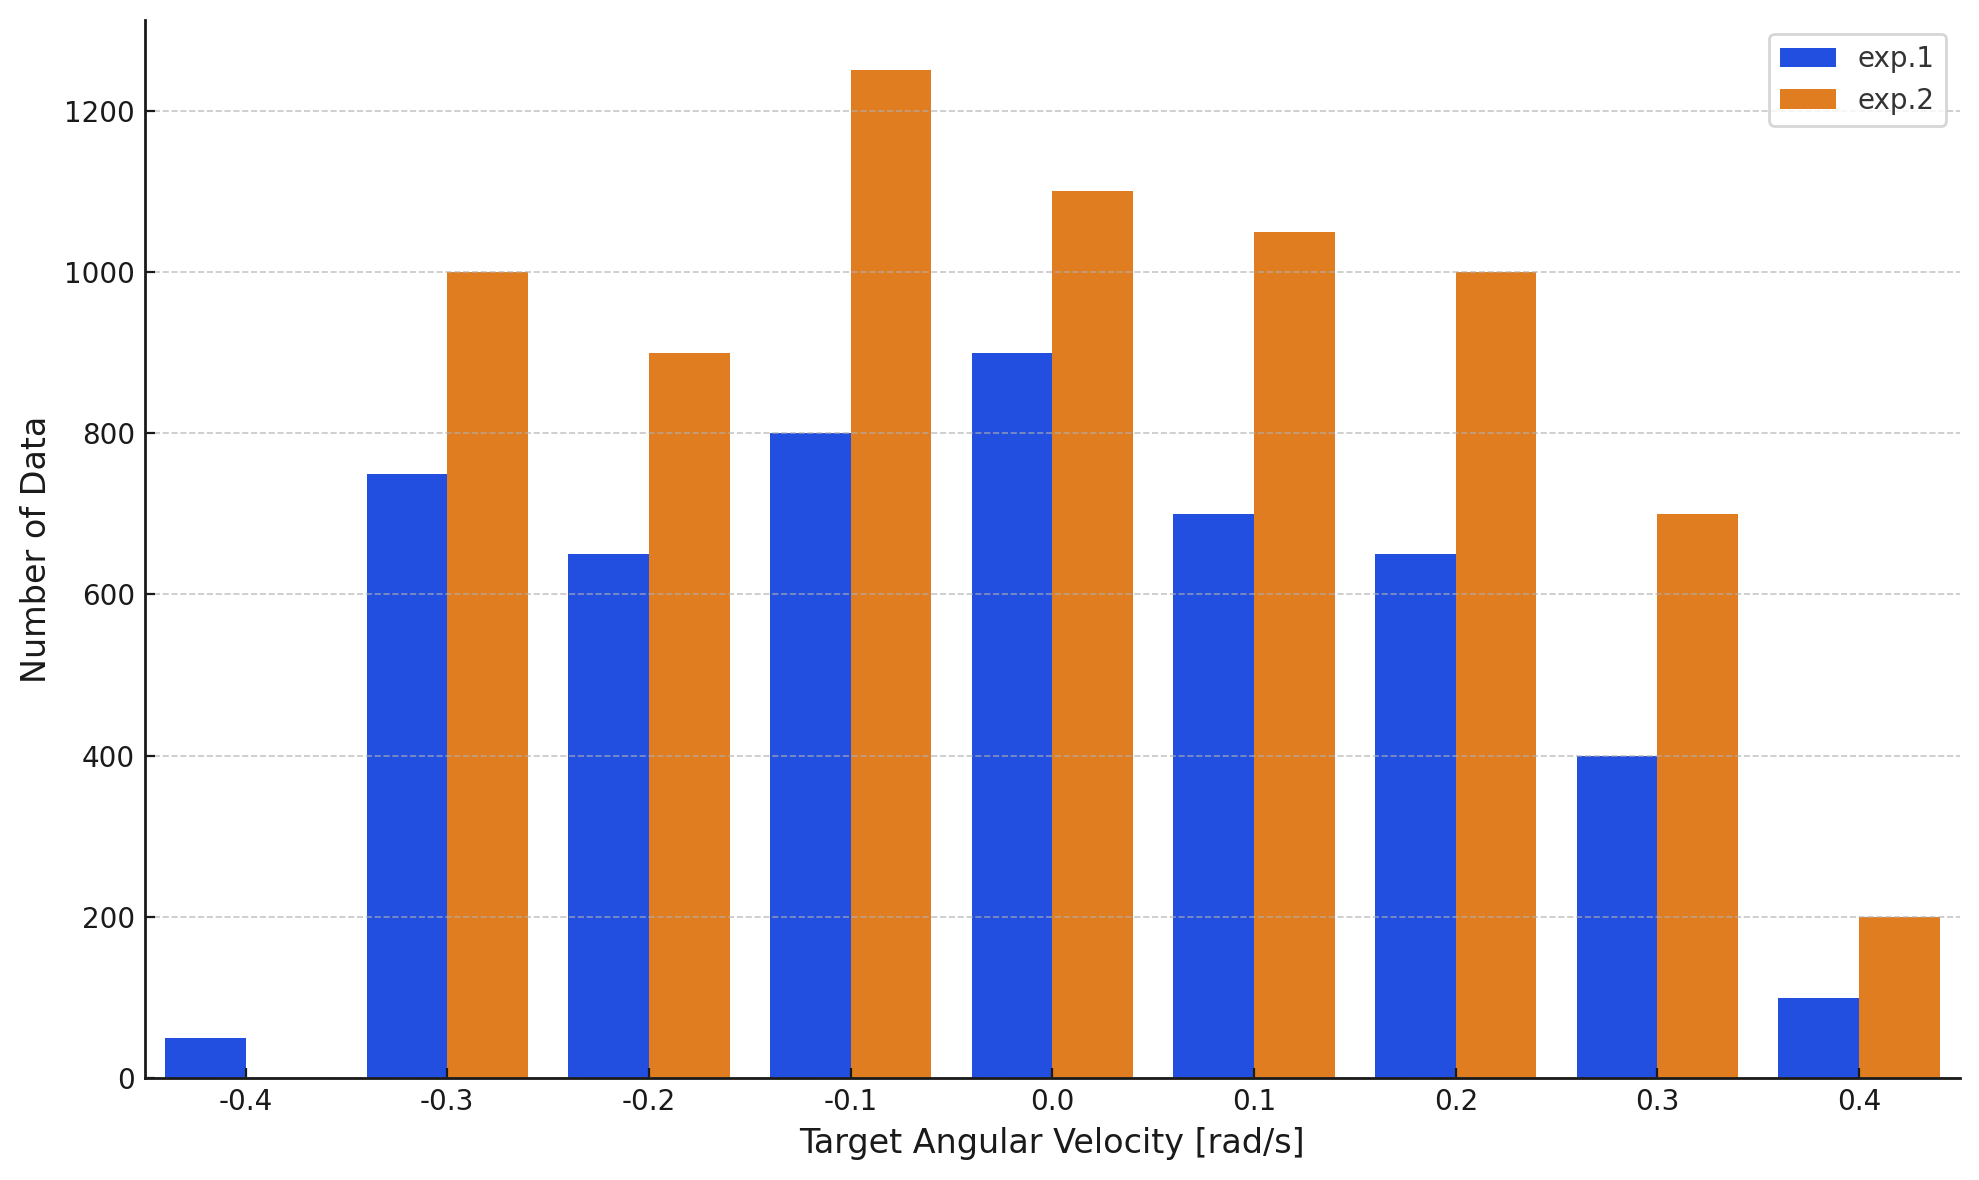
\includegraphics[keepaspectratio, scale=0.5]{images/output.png}
%   \caption{Comparison of target angular velocity ratios}
%   \label{Fig:ratio}
% \end{figure}

% 実験1と実験2の教師データを入れ替えて実験を行った. まず, 実験1のカメラ画像と実験2の目標角速度の組み合わせで学習を行った.